% ============================================================
\chapter{Conditions d'Optimalit\'e --- KKT}
\label{ch:kkt}
% ============================================================

En optimisation sans contraintes, la condition d'optimalit\'e est simple~: le gradient s'annule. Mais d\`es qu'on ajoute des contraintes --- in\'egalit\'es, \'egalit\'es --- cette condition na\"ive ne suffit plus. Les conditions de Karush-Kuhn-Tucker (KKT), d\'ecouvertes ind\'ependamment par William Karush en 1939 (dans un m\'emoire de master rest\'e longtemps ignor\'e) et par Harold Kuhn et Albert Tucker en 1951, g\'en\'eralisent la condition du gradient nul en introduisant les \emph{multiplicateurs de Lagrange} pour les contraintes. En optimisation convexe, sous des conditions de qualification tr\`es g\'en\'erales, les conditions KKT sont non seulement n\'ecessaires mais aussi \emph{suffisantes} --- elles caract\'erisent compl\`etement les solutions optimales.

\section{Introduction}

Les conditions de Karush--Kuhn--Tucker (KKT) g\'en\'eralisent la condition classique
$\nabla f(x^*) = 0$ aux probl\`emes d'optimisation avec contraintes. En optimisation
convexe, sous des conditions de qualification tr\`es g\'en\'erales, les conditions KKT
sont \`a la fois n\'ecessaires et suffisantes pour l'optimalit\'e.

\section{Probl\`eme d'optimisation convexe sous contraintes}

Consid\'erons le probl\`eme g\'en\'eral~:
\[
    \begin{aligned}
        & \min_{x \in \R^n} && f(x) \\
        & \text{sous} && g_i(x) \leq 0, \quad i = 1, \ldots, m, \\
        & && h_j(x) = 0, \quad j = 1, \ldots, p,
    \end{aligned}
    \tag{P}
\]
o\`u $f$ et les $g_i$ sont convexes et les $h_j$ sont affines~: $h_j(x) = a_j^T x - b_j$.

\begin{definition}[Ensemble r\'ealisable]
L'\emph{ensemble r\'ealisable} est~:
\[
    \mathcal{F} = \{x \in \R^n \mid g_i(x) \leq 0, \; i=1,\ldots,m, \;
    h_j(x) = 0, \; j=1,\ldots,p\}.
\]
\end{definition}

\begin{definition}[Contrainte active]
La contrainte $g_i(x) \leq 0$ est \emph{active} en $x$ si $g_i(x) = 0$.
L'ensemble des indices actifs est $\mathcal{A}(x) = \{i \mid g_i(x) = 0\}$.
\end{definition}

\section{Conditions KKT}

\begin{definition}[Conditions KKT]
Un point $x^* \in \mathcal{F}$ satisfait les \emph{conditions KKT} s'il existe des
multiplicateurs $\lambda^* \in \R^m$ et $\nu^* \in \R^p$ tels que~:
\begin{enumerate}
    \item \textbf{Stationnarit\'e}~:
    $\displaystyle 0 \in \partial f(x^*) + \sum_{i=1}^m \lambda_i^* \partial g_i(x^*)
    + \sum_{j=1}^p \nu_j^* a_j$.
    \item \textbf{R\'ealisabilit\'e primale}~: $g_i(x^*) \leq 0$ et $h_j(x^*) = 0$.
    \item \textbf{R\'ealisabilit\'e duale}~: $\lambda_i^* \geq 0$ pour tout $i$.
    \item \textbf{Compl\'ementarit\'e}~: $\lambda_i^* g_i(x^*) = 0$ pour tout $i$.
\end{enumerate}
\end{definition}

Si $f$ et les $g_i$ sont diff\'erentiables, la condition de stationnarit\'e s'\'ecrit~:
\[
    \nabla f(x^*) + \sum_{i=1}^m \lambda_i^* \nabla g_i(x^*) + \sum_{j=1}^p \nu_j^* a_j = 0.
\]

\begin{formules}[title=\textbf{Conditions KKT (cas diff\'erentiable)}]
\[
    \nabla f(x^*) + \sum_{i=1}^m \lambda_i^* \nabla g_i(x^*) + A^T\nu^* = 0, \quad
    \lambda^* \geq 0, \quad
    \lambda^* \circ g(x^*) = 0, \quad
    g(x^*) \leq 0, \quad
    Ax^* = b.
\]
\end{formules}

\begin{intuition}
La condition de compl\'ementarit\'e $\lambda_i^* g_i(x^*) = 0$ signifie que soit
la contrainte est inactive ($g_i(x^*) < 0$ et $\lambda_i^* = 0$), soit elle est
active ($g_i(x^*) = 0$ et $\lambda_i^* \geq 0$ potentiellement non nul).
Le multiplicateur $\lambda_i^*$ mesure la \og{}force\fg avec laquelle la contrainte
pousse la solution.
\end{intuition}

\section{Qualification des contraintes}

\begin{definition}[Condition de Slater]
La \emph{condition de Slater} est satisfaite s'il existe un point strictement
r\'ealisable $\hat{x}$ tel que~:
\[
    g_i(\hat{x}) < 0, \quad i = 1, \ldots, m, \quad
    h_j(\hat{x}) = 0, \quad j = 1, \ldots, p.
\]
(Pour les contraintes affines $g_i$, il suffit que $g_i(\hat{x}) \leq 0$.)
\end{definition}

\begin{theoreme}[KKT --- conditions n\'ecessaires et suffisantes]
\label{thm:kkt}
Consid\'erons le probl\`eme (P) avec $f, g_i$ convexes et $h_j$ affines.
\begin{enumerate}
    \item \textbf{Suffisance (toujours)}~: si $(x^*, \lambda^*, \nu^*)$ satisfait
    les conditions KKT, alors $x^*$ est une solution optimale de (P).
    \item \textbf{N\'ecessit\'e (sous Slater)}~: si la condition de Slater est
    satisfaite et $x^*$ est optimal, alors il existe $(\lambda^*, \nu^*)$ tel que
    $(x^*, \lambda^*, \nu^*)$ satisfait les conditions KKT.
\end{enumerate}
\end{theoreme}

\begin{proof}[Preuve de la suffisance]
Supposons que $(x^*, \lambda^*, \nu^*)$ satisfait KKT. Pour tout $x \in \mathcal{F}$~:
\begin{align*}
    f(x) &\geq f(x^*) + \inner{g_f}{x - x^*}
    \quad \text{o\`u } g_f \in \partial f(x^*) \\
    &= f(x^*) - \sum_i \lambda_i^* \inner{g_{g_i}}{x-x^*} - \sum_j \nu_j^* a_j^T(x-x^*)
    \quad \text{(stationnarit\'e)} \\
    &\geq f(x^*) - \sum_i \lambda_i^*(g_i(x) - g_i(x^*)) - \sum_j \nu_j^*(h_j(x) - h_j(x^*))
    \quad \text{(sous-gradient de } g_i) \\
    &\geq f(x^*) - \sum_i \lambda_i^* g_i(x) + \sum_i \lambda_i^* g_i(x^*)
    \quad \text{(car } h_j(x) = h_j(x^*) = 0) \\
    &\geq f(x^*) \quad \text{(car } \lambda_i^* \geq 0, g_i(x) \leq 0,
    \lambda_i^* g_i(x^*) = 0).
\end{align*}
\end{proof}

\section{Exemples d'application des conditions KKT}

\begin{exemple}[Programmation quadratique]
Consid\'erons~:
\[
    \min_x \frac{1}{2}x^TQx + c^Tx \quad \text{sous} \quad Ax \leq b.
\]
Les conditions KKT sont~:
\[
    Qx^* + c + A^T\lambda^* = 0, \quad \lambda^* \geq 0, \quad
    A x^* \leq b, \quad \lambda^* \circ (Ax^* - b) = 0.
\]
\end{exemple}

\begin{exemple}[Projection sur un convexe]
La projection $\bar{x} = \mathrm{proj}_C(y)$ r\'esout~:
\[
    \min_x \frac{1}{2}\norm{x - y}^2 \quad \text{sous} \quad x \in C.
\]
Si $C = \{x \mid g_i(x) \leq 0\}$, les conditions KKT donnent~:
\[
    \bar{x} - y + \sum_i \lambda_i^* \nabla g_i(\bar{x}) = 0, \quad
    \lambda_i^* \geq 0, \quad \lambda_i^* g_i(\bar{x}) = 0.
\]
\end{exemple}

\begin{exemple}[SVM \`a marge dure]
Le SVM primal~:
\[
    \min_{w,b} \frac{1}{2}\norm{w}^2 \quad \text{sous} \quad
    y_i(\inner{w}{x_i} + b) \geq 1, \; i=1,\ldots,N.
\]
Les conditions KKT~:
\[
    w^* = \sum_i \alpha_i^* y_i x_i, \quad
    \sum_i \alpha_i^* y_i = 0, \quad
    \alpha_i^* \geq 0, \quad
    \alpha_i^*(y_i(\inner{w^*}{x_i} + b^*) - 1) = 0.
\]
La compl\'ementarit\'e montre que seuls les points avec $y_i(\inner{w^*}{x_i} + b^*) = 1$
(vecteurs de support) ont $\alpha_i^* > 0$.
\end{exemple}

\section{Interpr\'etation g\'eom\'etrique}

\begin{center}
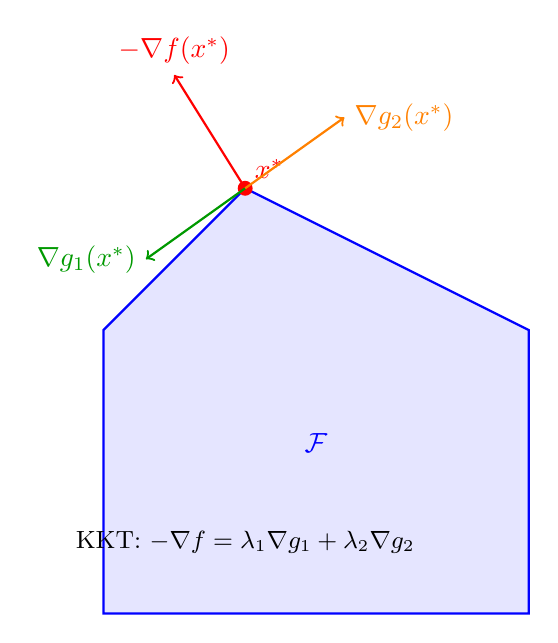
\begin{tikzpicture}[scale=1.8]
    % Feasible region
    \fill[blue!10] (0,0) -- (3,0) -- (3,2) -- (1,3) -- (0,2) -- cycle;
    \draw[thick, blue] (0,0) -- (3,0) -- (3,2) -- (1,3) -- (0,2) -- cycle;

    % Optimal point
    \fill[red] (1,3) circle (1.5pt) node[above right] {$x^*$};

    % Gradient of f
    \draw[->, thick, red] (1,3) -- (0.5,3.8) node[above] {$-\nabla f(x^*)$};

    % Constraint gradients
    \draw[->, thick, green!60!black] (1,3) -- (0.3,2.5) node[left] {$\nabla g_1(x^*)$};
    \draw[->, thick, orange] (1,3) -- (1.7,3.5) node[right] {$\nabla g_2(x^*)$};

    % Labels
    \node[blue] at (1.5,1.2) {$\mathcal{F}$};
    \node at (1, 0.5) {\small KKT: $-\nabla f = \lambda_1 \nabla g_1 + \lambda_2 \nabla g_2$};
\end{tikzpicture}
\end{center}

\section{Autres qualifications de contraintes}

\begin{definition}[Ind\'ependance lin\'eaire (LICQ)]
La \emph{LICQ} est satisfaite en $x^*$ si les gradients des contraintes actives
$\{\nabla g_i(x^*)\}_{i \in \mathcal{A}(x^*)} \cup \{a_j\}_{j=1}^p$ sont
lin\'eairement ind\'ependants.
\end{definition}

\begin{proposition}
Sous LICQ, les multiplicateurs KKT sont uniques.
\end{proposition}

\begin{definition}[Qualification de Mangasarian--Fromovitz (MFCQ)]
La \emph{MFCQ} est satisfaite en $x^*$ si les $\{a_j\}$ sont lin\'eairement
ind\'ependants et il existe $d \in \R^n$ tel que~:
\[
    \inner{\nabla g_i(x^*)}{d} < 0, \; \forall i \in \mathcal{A}(x^*), \quad
    a_j^T d = 0, \; \forall j.
\]
\end{definition}

\section{Sensibilit\'e et interpr\'etation \'economique}

\begin{theoreme}[Sensibilit\'e]
\label{thm:sensibilite}
Soit $p^*(u, v)$ la valeur optimale du probl\`eme perturb\'e~:
\[
    \min f(x) \quad \text{sous} \quad g_i(x) \leq u_i, \; h_j(x) = v_j.
\]
Sous des conditions de r\'egularit\'e, les multiplicateurs KKT satisfont~:
\[
    \lambda_i^* = -\frac{\partial p^*}{\partial u_i}\bigg|_{(0,0)}, \quad
    \nu_j^* = -\frac{\partial p^*}{\partial v_j}\bigg|_{(0,0)}.
\]
\end{theoreme}

\begin{remarque}
$\lambda_i^*$ repr\'esente le \og{}prix marginal\fg de la $i$-\`eme contrainte~:
rel\^acher la contrainte d'une unit\'e am\'eliore la valeur optimale de $\lambda_i^*$.
\end{remarque}

\section{Impl\'ementation Python}

\begin{codeblock}[title=\textbf{V\'erification des conditions KKT avec CVXPY}]
\begin{minted}{python}
import numpy as np
import cvxpy as cp

# Programmation quadratique
n = 5
np.random.seed(42)
Q = np.random.randn(n, n)
Q = Q.T @ Q + 0.1 * np.eye(n)  # PD
c = np.random.randn(n)
A = np.random.randn(3, n)
b = np.ones(3)

x = cp.Variable(n)
constraints = [A @ x <= b]
prob = cp.Problem(cp.Minimize(0.5 * cp.quad_form(x, Q) + c @ x),
                  constraints)
prob.solve()

x_star = x.value
lambda_star = constraints[0].dual_value

print("Solution x*:", x_star)
print("Multiplicateurs lambda*:", lambda_star)

# Verification stationnarite
grad_L = Q @ x_star + c + A.T @ lambda_star
print(f"||grad L|| = {np.linalg.norm(grad_L):.2e}")

# Verification complementarite
slack = b - A @ x_star
comp = lambda_star * slack
print(f"Complementarite: max|lambda*g| = {np.max(np.abs(comp)):.2e}")

# Verification faisabilite
print(f"Faisabilite primale: max(Ax-b) = {np.max(A @ x_star - b):.2e}")
print(f"Faisabilite duale: min(lambda) = {np.min(lambda_star):.2e}")
\end{minted}
\end{codeblock}

\section{Exercices}

\begin{exercice}[$\star$]
R\'esoudre $\min x_1^2 + x_2^2$ sous $x_1 + x_2 \geq 1$ en utilisant les conditions KKT.
\end{exercice}

\begin{exercice}[$\star$]
V\'erifier que la condition de Slater est satisfaite pour
$\min \norm{x}^2$ sous $\norm{x}_\infty \leq 1$.
\end{exercice}

\begin{exercice}[$\star\star$]
D\'eriver les conditions KKT du probl\`eme SVM \`a marge souple~:
\[
    \min_{w,b,\xi} \frac{1}{2}\norm{w}^2 + C\sum_i \xi_i \quad \text{sous} \quad
    y_i(\inner{w}{x_i} + b) \geq 1 - \xi_i, \; \xi_i \geq 0.
\]
\end{exercice}

\begin{exercice}[$\star\star$]
Montrer que pour un probl\`eme de programmation lin\'eaire, les conditions KKT
sont \'equivalentes aux conditions de compl\'ementarit\'e primale-duale.
\end{exercice}

\begin{exercice}[$\star\star\star$]
D\'emontrer le th\'eor\`eme de sensibilit\'e~\ref{thm:sensibilite} pour un
probl\`eme de programmation lin\'eaire.
\end{exercice}

\begin{exercice}[$\star\star\star$]
Montrer que sous la condition LICQ, les multiplicateurs KKT sont uniques.
Donner un exemple o\`u LICQ n'est pas satisfaite et les multiplicateurs ne
sont pas uniques.
\end{exercice}
